	% !TEX TS-program = pdflatex
	% !TEX encoding = UTF-8 Unicode
	
	% This is a simple template for a LaTeX document using the "article" class.
	% See "book", "report", "letter" for other types of document.
	
	\documentclass[11pt]{article} % use larger type; default would be 10pt
	
	\usepackage[utf8]{inputenc} % set input encoding (not needed with XeLaTeX)
	
	%%% Examples of Article customizations
	% These packages are optional, depending whether you want the features they provide.
	% See the LaTeX Companion or other references for full information.
	
	%%% PAGE DIMENSIONS
	\usepackage{geometry} % to change the page dimensions
	\geometry{a4paper} % or letterpaper (US) or a5paper or....
	% \geometry{margin=2in} % for example, change the margins to 2 inches all round
	% \geometry{landscape} % set up the page for landscape
	%   read geometry.pdf for detailed page layout information
	
	\usepackage{graphicx} % support the \includegraphics command and options
	
	% \usepackage[parfill]{parskip} % Activate to begin paragraphs with an empty line rather than an indent
	
	%%% PACKAGES
	\usepackage{booktabs} % for much better looking tables
	\usepackage{array} % for better arrays (eg matrices) in maths
	\usepackage{paralist} % very flexible & customisable lists (eg. enumerate/itemize, etc.)
	\usepackage{verbatim} % adds environment for commenting out blocks of text & for better verbatim
	\usepackage{subfig} % make it possible to include more than one captioned figure/table in a single float
	\usepackage{graphicx}
	% These packages are all incorporated in the memoir class to one degree or another...
	
	%%% HEADERS & FOOTERS
	\usepackage{fancyhdr} % This should be set AFTER setting up the page geometry
	\pagestyle{fancy} % options: empty , plain , fancy
	\renewcommand{\headrulewidth}{0pt} % customise the layout...
	\lhead{}\chead{}\rhead{}
	\lfoot{}\cfoot{\thepage}\rfoot{}
	
	%%% SECTION TITLE APPEARANCE
	\usepackage{sectsty}
	\allsectionsfont{\sffamily\mdseries\upshape} % (See the fntguide.pdf for font help)
	% (This matches ConTeXt defaults)
	
	%%% ToC (table of contents) APPEARANCE
	\usepackage[nottoc,notlof,notlot]{tocbibind} % Put the bibliography in the ToC
	\usepackage[titles,subfigure]{tocloft} % Alter the style of the Table of Contents
	\renewcommand{\cftsecfont}{\rmfamily\mdseries\upshape}
	
	%%% END Article customizations
	
	%%% The "real" document content comes below...
	
	\title{Documentaci\'on Base de datos}
	\author{David G\'omez S\'anchez y Pablo Vicente Munuera}
	\date{} % Activate to display a given date or no date (if empty),
	         % otherwise the current date is printed 
	
	\begin{document}
	\maketitle
	
	\begin{abstract}
	
	Este documento contiene lo necesario para la creación de una base de datos relacional en PostgreSQL en la que se almacenarán datos provenientes de PFAM, JGI y HMMER3 para la posterior obtención de información concerniente a proteínas del organismo \emph{Pseudovirgaria hyperparasitica}.
	
	\end{abstract}
	
	\section{Getting started}
	
	Aunque est\'a explicado como preparar el entorno para ejecutar nuestros programas, procederemos a hacerlo, igualmente, aqu\'i.
	
	\subsection{Inserción de las tablas en la base de datos y ejecución del programa principal (main.py):}
	
	Lo primero que debe hacer es ejecutar, en una terminal, el script para acceder a la base de datos y crear las tablas necesarias para la ejecución de los programas:
	
	\textbf{chmod a+x init.sh}
	
	\textbf{./init.sh}
	
	NOTA: los valores por defecto para psql son: localhost:5432:masterdb:masteruser:masterpass, si desea cambiarlos, por favor modifique el archivo init.sh
	
	Realizado el primer paso, se deberá ejecutar el programa, escribiendo lo siguiente en una terminal:
	
	\textbf{python3.4 ~/main.py}
	
	Una vez dentro, observaremos un menú en pantalla que nos da la opción de escoger entre diferentes opciones. El usuario deberá seleccionar las tres primeras en orden, para despues poder optar a seleccionar las siguientes.
	Esto se debe a que las tres primeras opciones son programas de tipo analizador sintáctico de patrones (parser) capaces de obtener datos desde JGI(opción 1), PFAM(opción 2) y HMMER3 (opción 3) para acto seguido insertarlos en las tablas creadas en nuestra base de datos, mientras que los programas siguientes sirven para obtener información de dichas tablas una vez realizados los pasos 1, 2 y 3.
	
	NOTA: se requerirá de un parámetro en las opciones 1,2 y 3 para los cuales el usuario puede indicar la ruta de los ficheros a introducir, o teclear 'intro', lo que introduce la ruta por defecto:
	
	\begin{itemize}
	
	\item \emph{Datasets/Psehy1\_GeneCatalog\_proteins\_20140829.aa.fasta} (Opción 1)
	
	\item \emph{Datasets/Pfam-A.seed} (Opción 2)
	
	\item \emph{Datasets/Pfam-A.hmm} (Opción 3)
	
	\end{itemize}
	
	\subsection{Programas de consulta a la base de datos:}
	
	En este apartado se describen los programas que realizan consultas SQL a la base de datos (opciones 4-6 resultantes de la ejecución del programa principal \textbf{main.py}

\begin{itemize}

\item Opción 4: Programa que muestra por pantalla los dominios de las proteínas analizadas. Necesita como parámetro una proteína del organismo \emph{Pseudovirgaria hyperparasitica} (ID o descripción de JGI) tecleada directamente en la terminal.

\item Opción 5: Programa que muestra por pantalla los identificadores de InterPro  de las proteínas analizadas. Necesita como parámetro una proteína del organismo \emph{Pseudovirgaria hyperparasitica} (ID o descripción de JGI) tecleada directamente en la terminal.

\item Opción 6: Programa que muestra por pantalla, para las proteínas etiquetadas como \textbf{kinasas, lyasas, canales iónicos, receptores} o \textbf{transportadores}, el número medio, máximo, mínimo y desviación estándar del número de dominios de  \emph{Pseudovirgaria hyperparasitica} . En este caso no es necesario ningún parámetro en la ejecución del mismo.

\end{itemize}

\section{Realizaci\'on de la pr\'actica}

\subsection{Herramientas utilizadas}

\begin{itemize}

\item Sublime Text o Geany. David utilizó Geany, mientras que Pablo utilizó Sublime Text, por cuestión de gustos, cumpliendo ambos perfectamente su función.

\item Texworks. Es el programa utilizado para editar los textos de latex. Tiene funci\'on de compilado y te muestra en una ventana aparte el pdf generado.

\item Github. Hemos utilizado un control de versiones digno, ya que en la experiencia de Pablo, es infinitamente mejor trabajar con uno, que trabajar sin \'el. David nunca hab\'ia utilizado uno, pero en seguida le ha pillado el tranquillo y est\'a muy agusto trabajando de esta manera.

\item Python3.4. Es el lenguaje y versi\'on establecida por el profesorado, debíamos ajustarnos a \'el.

\item Postgresql. Hab\'ia la posibilidad de utilizar SQLite, pero preferimos utilizar PostGreSQL debido a que nos parecía mas engorroso utilizar un gestor de bases de datos embebido para una práctica como esta.

\end{itemize}

\subsection{Organizaci\'on del trabajo}

Aunque lo ideal hubiera sido utilizar \emph{pair-programming} para la realizaci\'on de esta pr\'actica, se ha optado por repartirnos el trabajo e intentar quedar lo m\'aximo posible para que no hubiera dudas, ni problemas, de modo que no se retrasara la velocidad de trabajo. B\'asicamente hemos intentado hacer ambos miembros de la pr\'actica, tanto algo de lo que ser\'ia m\'as bases de datos (consultas, dise\~no, etc...), como algo de la parte de programaci\'on, aprendiendo as\'i las partes necesarias que se requer\'ian para esta asignatura.

\subsection{Dise\~no de base de datos}

El dise\~no de base de datos nos ha llevado de cabeza durante la mayor parte del desarrollo del trabajo, aunque eso trataremos m\'as debidamente en la secci\'on: problemas encontrados.

Ha habido dos tablas claras desde el primero momento: la tabla jgi y la tabla Pfam. La primera representa al punto 1.a ''Procedente de jgi'' y corresponde a las prote\'inas y sus correspondientes secuencias y datos. Tiene como clave primaria el id, lo cual parece l\'ogico, ya que es el elemento m\'as representativo de cada prote\'ina. Aunque en un primer momento se puso tambi\'en el organismo, posteriormente se vi\'o que el id cambiaba con el organismo, con lo que no era necesaria la dupla id-organismo como clave primaria. Al no tener algo en lo que basarnos para decidir los tipos, se ha tomado algo que no consumiera demasiado, pero que fuera m\'as que suficiente. Por ello, en cosas que pueden ser muy largas, como la secuencia y la descripci\'on, se han puesto \emph{Text} como tipo de dato. Los \emph{NOT NULL}, a\'un a sabiendas de que todo se deb\'ia meter, hay cosas que creemos que aunque no se metieran, no tendr\'ian un efecto adverso, a la hora de las b\'usquedas y filtrados.

Por otro lado, la tabla Pfam tambi\'en qued\'o bastante resuelta desde un principio. A parte de los datos que se nos informaba que deb\'ia contener esta tabla, lo \'unico que hab\'ia que pensar era la clave primaria y la posibilidad de claves alternativas. Las dos \'unicas cosas que no se pueden repetir es el ID y el accesion number. La combinaci\'on de ambas no era posible, ya que no para un mismo ID no va a haber 2 accesion number distintos, ser\'a siempre el mismo, con lo que se opta por poner una clave primaria (ID, pero podr\'ia haber sido perfectamente el accesion number) y una clave alternativa que ser\'a el accesion number. Los tipos de esta tabla, excepto el ID, que debi\'o adecuarse a otra tabla, estaban espec\'ificados en la p\'agina web oficial de Pfam, as\'i que no tuvimos que realizar el esfuerzo nosotros. Un dato curioso: intentando imitar lo que se di\'o en clase, se hizo una tabla para los accesion number y los posibles accesion numbers antiguos. Esta se acab\'o por eliminar, ya que no ten\'ia mucho sentido en el entorno de la pr\'actica.

El problema y la parte de las tablas que m\'as cambios han sufrido han sido las  correspondiente al punto 1.c ''Datos provenientes de hmmer''. Ha llegado a haber hasta 3 tablas, s\'olo para esta secci\'on. Finalmente, se vi\'o que con solo 2 tablas era suficiente. En primer lugar, tenemos la tabla hmmer, en la cual, guardamos la informaci\'on de: el ID de la prote\'ina con la que hacemos la query a hmmscan, que ser\'a un \emph{INT} ya que es un n\'umero; la descripci\'on de esta, que no tendr\'a  tope de caracteres; y el e-value que debido a que puede ser muy peque\~no, lo pondremos como \emph{float}. El ID de esta tabla ser\'a clave primaria y har\'a referencia al mismo ID de JGI. Por lo tanto, en la tabla HMMER deber\'an existir solo los ID, los cuales se encuentren tambi\'en almacenados en la tabla JGI. 

La tabla Domains, deber\'ia tener un apartado a parte en la secci\'on de problemas. Solo esta tabla ha sufrido m\'as cambios que todas las dem\'as juntas. Esto es debido en gran parte a que no ten\'iamos la experiencia necesaria, y hasta que no supimos como afrotar y que debiamos hacer en el punto 2.3 (e incluso en mitad del desarrollo) no supimos el correcto dise\~no de dicha tabla. En un principio iban a ser dos tablas, pero al final, qued\'o reducida a un \'unica tabla. En ella tendriamos, el ID del dominio, que ser\'a, b\'asicamente, un autogenerado que en postgreSQL se denomina \emph{serial}, el cual ser\'a clave primaria. Como datos \emph{INT} tenemos: startAA, que corresponde al n\'umero d\'onde empieza el amino\'acido alineado del dominio; endAA, es la posici\'on d\'onde acaba el alineamiento; y el score, que es la puntuaci\'on obtenida en el alineamiento (como es de bueno o malo). Tambi\'en tenemos como elemento \emph{float}, el evalueInd, que corresponde al independent e-value. Estos datos eran lo que se ped\'ia en la segunda parte del punto 1.c. Para que se relacionasen estos datos tanto con la tabla Hmmer, como con los datos en Pfam, debemos a\~nadir tres campos m\'as, correspodientes a: La prote\'ina query, representada por IDQuery que hace referencia a la columna ID de Hmmer, la cual, a su vez, llevar\'a a la prote\'ina de JGI; Los dominios target, que referencian a la tabla Pfam, y, por lo tanto, tendremos que tener sus correspondientes valores, AccTarget (accesion number del dominio) y NameTarget (ID de Pfam). Ambas relaciones ser\'an de 1 a 1 desde la tabla Domains hacia las otras tablas.


\begin{figure}
\centering
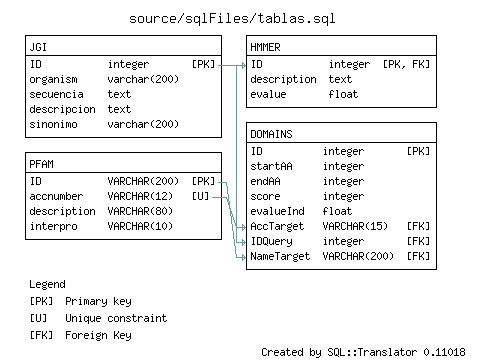
\includegraphics[width=15cm]{design}
\caption{Dise\~no final de la base de datos\label{fig:Design}}
\end{figure}

\subsection{Problemas encontrados}

\subsubsection{Problemas con python y SQL}

En mi caso (David, perfil bio) he tenido ciertos problemas a la hora de enfrentarme a la sintaxis del código en python y saber resolver programas de parseo, por simple deficiencia en conocimientos de programación, que finalmente han sido subsanados en su gran mayoría por el compañero Pablo. Por otra parte, ciertas sentencias de SQL me han llevado algo de tiempo por el mismo motivo; sin embargo me he apoyado en Pablo, en el manual de PostgreSQL y en algún foro del tipo stackoverflow para sacarle mas partido y ampliar conocimientos, con lo que siento que he aprendido bastante.

\subsubsection{Problemas con el dise\~no de las tablas}

Como ya se ha mencionado anteriormente, la parte de las tablas correspondientes a la informaci\'on sacada desde \emph{hmmscan}, ha sido siempre la m\'as compleja y cambiante a lo largo del proyecto. En un primer momento se pens\'o que deb\'ia haber tres trablas: una para hmmer (eso no ha cambiado), y dos para los dominios. Esta se completaba con la informaci\'on b\'asica de un dominio en una tabla denominada dominio y otra tabla con las relaciones oportunas con pfam y hmmer (que ser\'ia la tabla domains). Pero, esto ten\'ia una pega, no merec\'ia la pena tener dos tablas, cuando en una sola, podr\'ias tener las dos y sin apenas redundancia, con lo que se decidi\'o ponerla en una sola.
A parte de los m\'ultiples cambios que han sufrido esta tablas, lo dem\'as no ha tenido mayor complejidad. 

\section{Conclusi\'on}

Como conclusi\'on podemos decir que la pr\'actica ha ayudado a la parte biol\'ogica a aumentar sus habilidades program\'aticas y afrontar problemas que antes no se les hab\'ian planteado. Para la parte inform\'atica, ha sido \'util para refrescar conceptos olvidados y para ver como se aplican conceptos inform\'aticos en temas biol\'ogicos.

\end{document}
